\documentclass[24pt, a0papper, portrait]{tikzposter}
\makeatletter
\def\title#1{\gdef\@title{\scalebox{\TP@titletextscale}{%
\begin{minipage}[t]{\linewidth}
\centering
#1
\par
\vspace{0.5em}
\end{minipage}%
}}}
\makeatother
\usepackage[utf8]{inputenc}
\usepackage{subfig}
\graphicspath{ {./images/} }
 
\title{Simulation of Various Channelizer Structures 
       Directed by Cyclostationary Detector}
\author{Brian H. Hulette, Amir I. Zaghloul}
\institute{Virginia Tech Dept. of Electrical Engineering}
 
\usetheme{Autumn}
 
\begin{document}
 
\maketitle

\begin{columns}
    \column{0.33}
    \block{Introduction}
    {
        \begin{tikzfigure}[Using polyphase analysis and synthesis channelizers together to create a highly configurable and efficient filter bank.]
            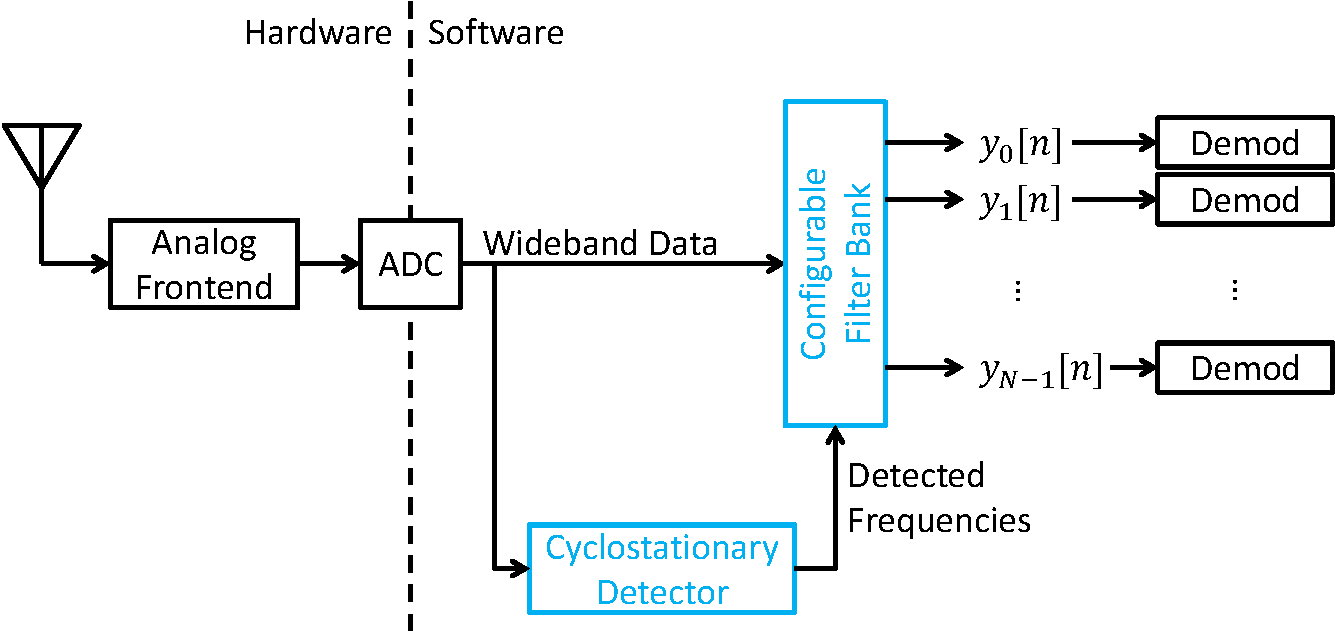
\includegraphics[width=\linewidth]{block_diagram}
        \end{tikzfigure}
    }
 
    \block{Cyclostationary Detection}
    {
        \begin{tikzfigure}[SCD Estimates for three signals at 156.25, 312.5, and 625 kbaud. SCD at $\alpha = 0$ Hz is equivalent to PSD, SCD at $\alpha=625$ Hz highlights signal at that baud rate.]
        \begin{minipage}[b]{0.45\linewidth}
            \centering
            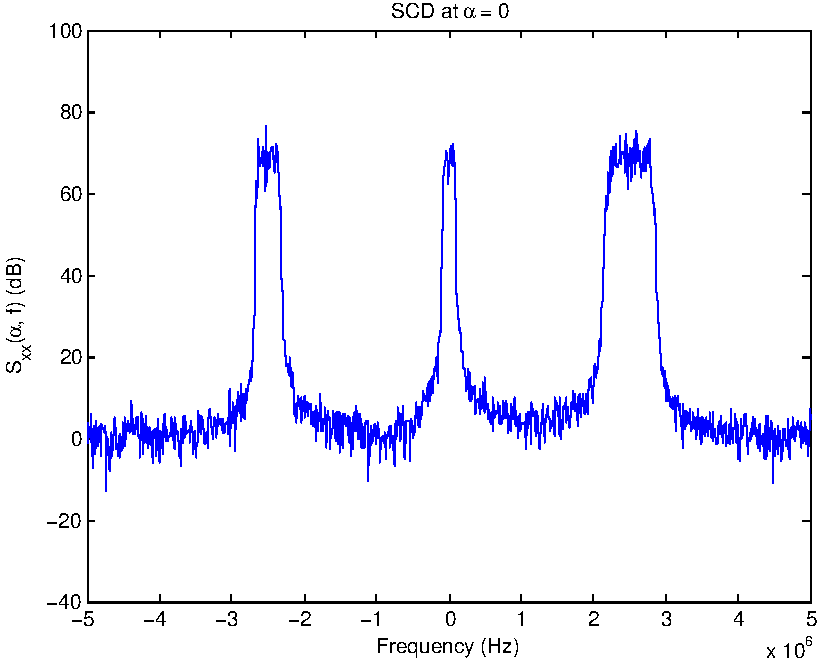
\includegraphics[width=\textwidth]{cyclo_0}
        \end{minipage}
        %\hspace{0.5cm}
        %\begin{minipage}[b]{0.45\linewidth}
        %    \centering
        %    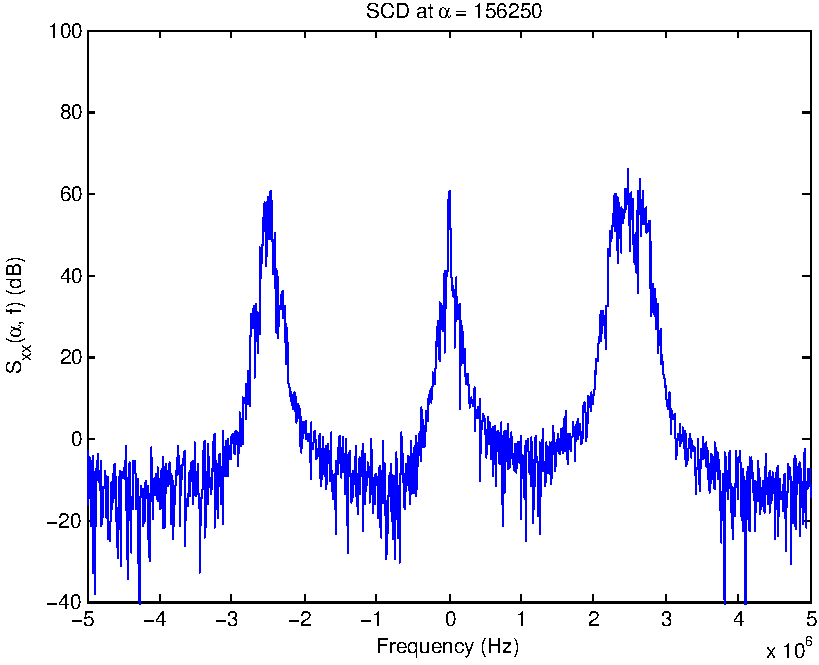
\includegraphics[width=\textwidth]{cyclo_156250}
        %    \label{fig:figure2}
        %\end{minipage}
        %\begin{minipage}[b]{0.45\linewidth}
        %    \centering
        %    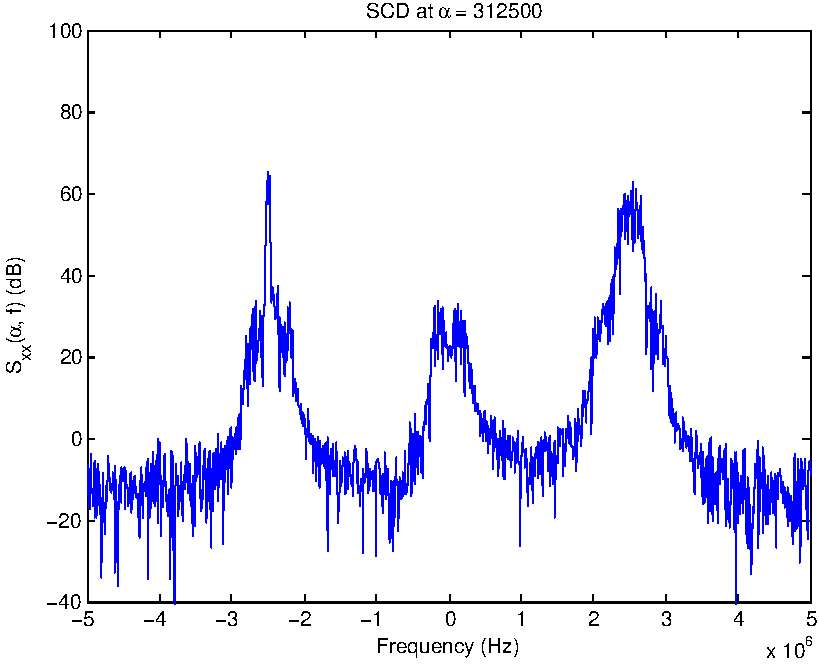
\includegraphics[width=\textwidth]{cyclo_312500}
        %    \label{fig:figure1}
        %\end{minipage}
        \hspace{0.5cm}
        \begin{minipage}[b]{0.45\linewidth}
            \centering
            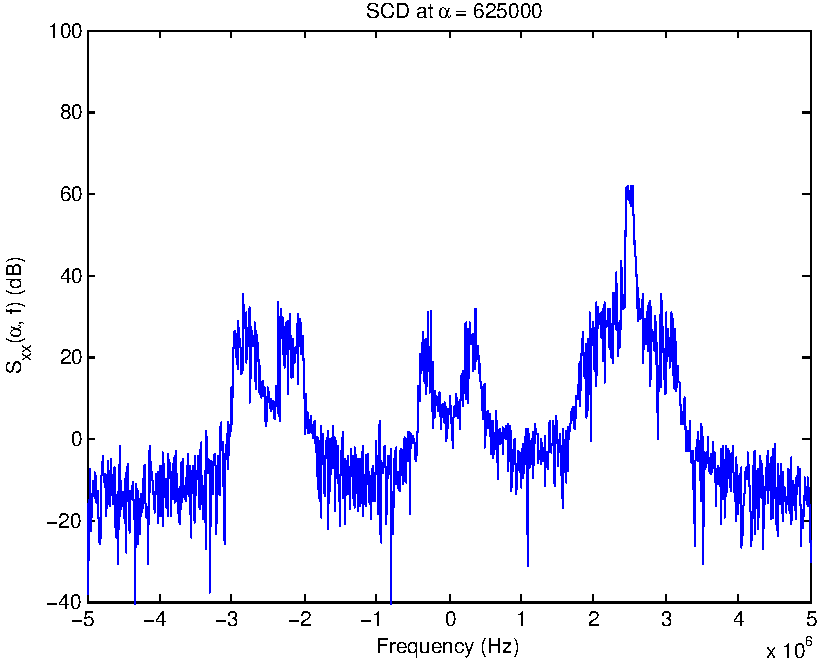
\includegraphics[width=\textwidth]{cyclo_625000}
        \end{minipage}
        \label{fig:scd}
        \end{tikzfigure}
    }
    \column{0.33}
    \block{Polyphase Filter Bank}
    {
        \begin{tikzfigure}[Non-maximally decimated ($D=M/2$) polyphase analysis and synthesis channelizers]
        \begin{minipage}[b]{\linewidth}
            \centering
            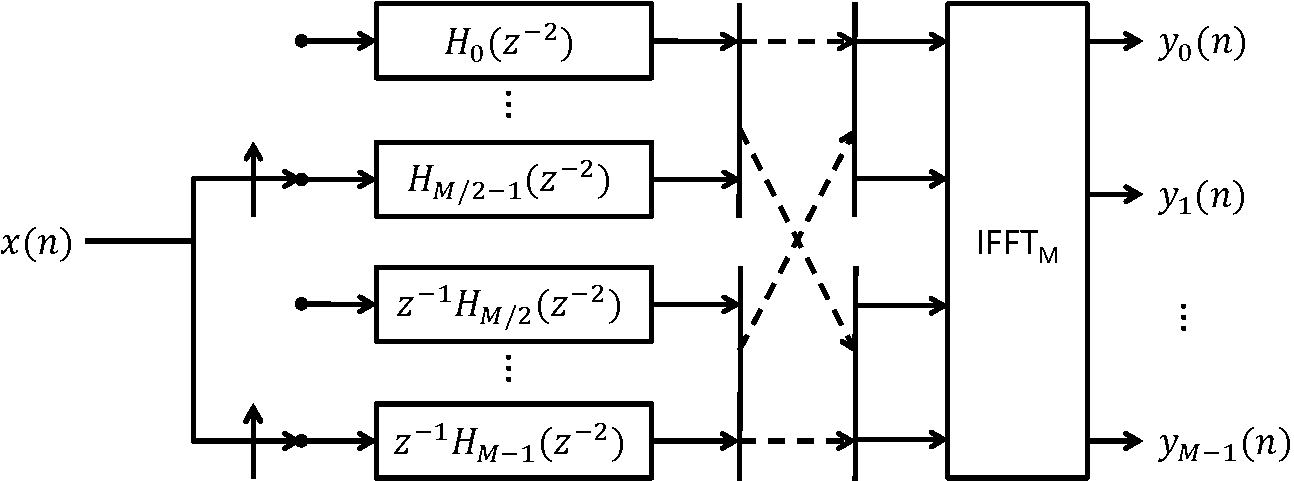
\includegraphics[width=0.45\textwidth]{polyphase_analysis_nmdfb}
        \end{minipage}
        \hspace{0.5cm}
        \begin{minipage}[b]{\linewidth}
            \centering
            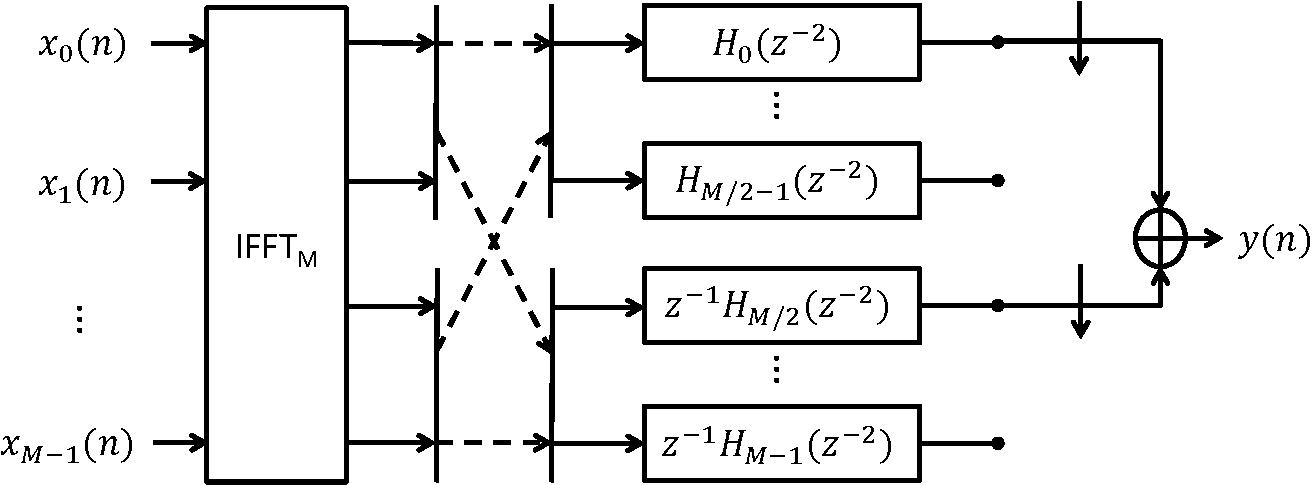
\includegraphics[width=0.45\textwidth]{polyphase_synthesis_nmdfb}
        \end{minipage}
        \label{fig:scd}
        \end{tikzfigure}
        \begin{tikzfigure}[Using polyphase analysis and synthesis channelizers together to create a highly configurable and efficient filter bank.]
            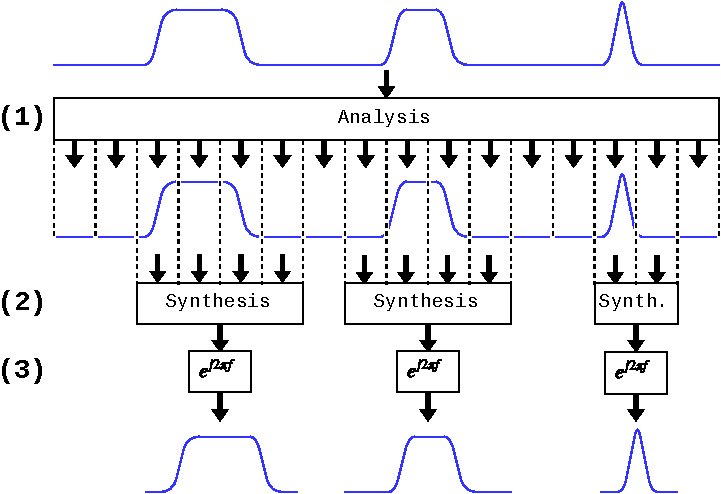
\includegraphics[width=\linewidth]{polyphase}
        \end{tikzfigure}

    }
    \block{Overlap-Save Filter Bank}
    {
        \begin{tikzfigure}[Using polyphase analysis and synthesis channelizers together to create a highly configurable and efficient filter bank.]
            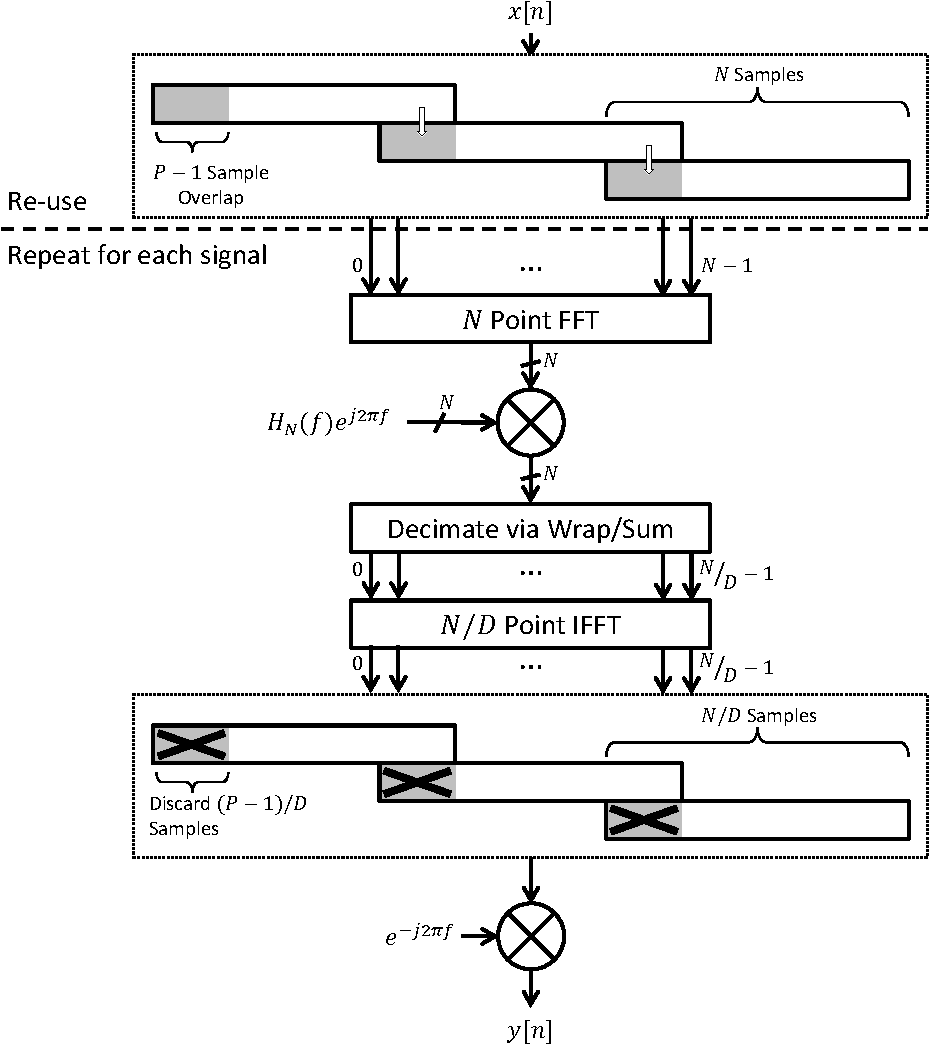
\includegraphics[width=\linewidth]{overlap_save_time_domain}
        \end{tikzfigure}
    }
    \column{0.33}
    \block{Simulation Results}
    {
        \begin{tikzfigure}[SCD Estimates for three signals at 156.25, 312.5, and 625 kbaud. SCD at $\alpha = 0$ equivalent to PSD.]
            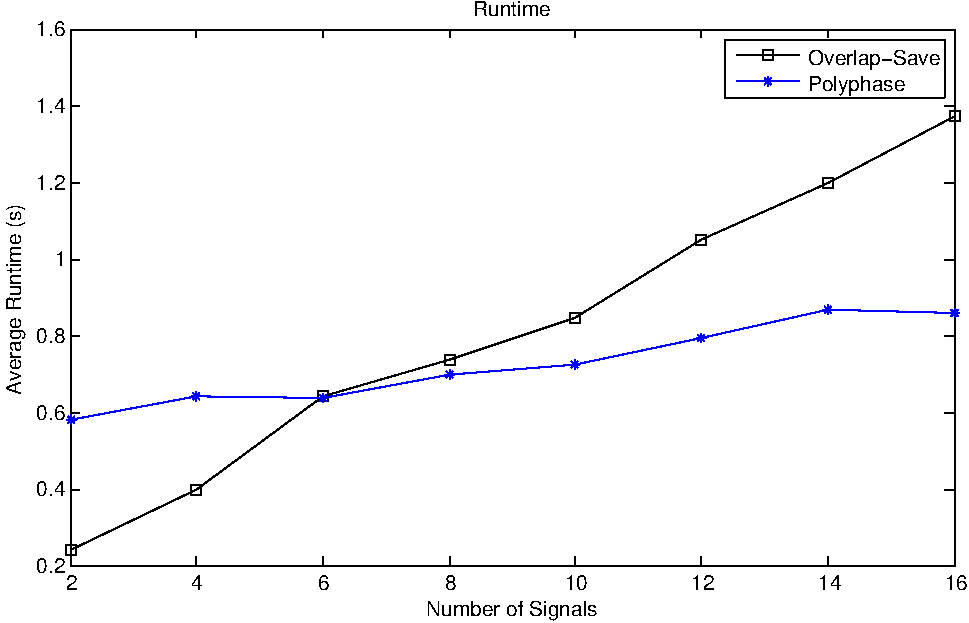
\includegraphics[width=\linewidth]{runtime_comparison_250}
        \end{tikzfigure}
        \begin{tikzfigure}[SCD Estimates for three signals at 156.25, 312.5, and 625 kbaud. SCD at $\alpha = 0$ equivalent to PSD.]
            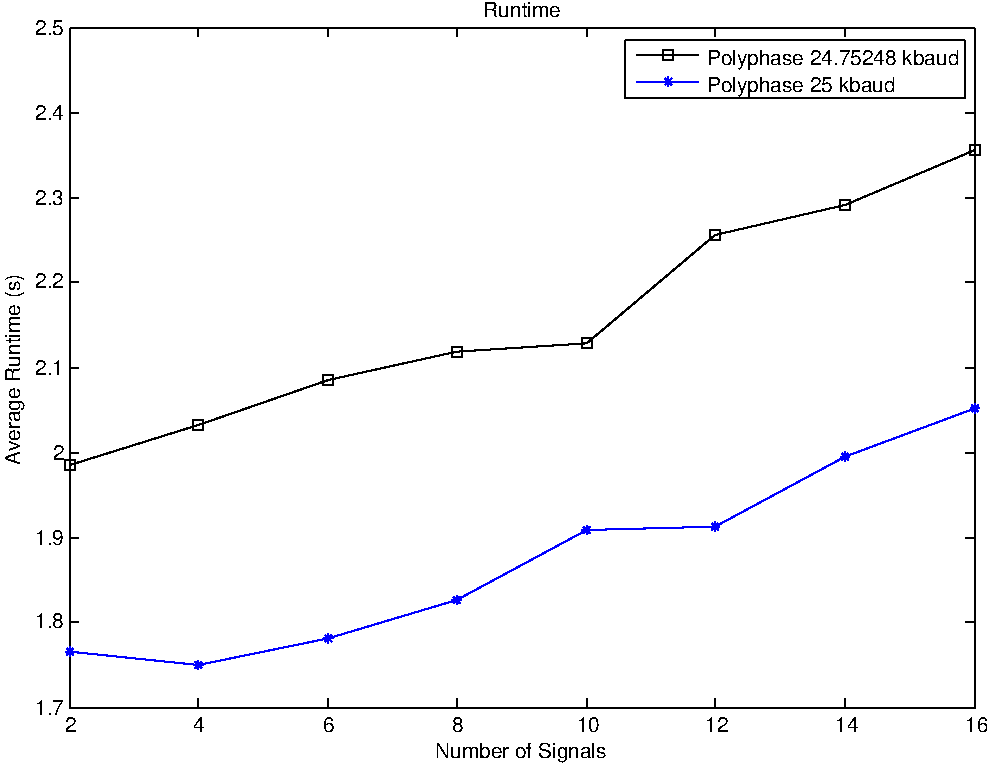
\includegraphics[width=\linewidth]{fft_runtime_comparison}
        \end{tikzfigure}
    }
\end{columns}
 
 
\end{document}
 
\end{document}
